\documentclass[a4paper]{article}
\usepackage[utf8]{inputenc}
%Pacote de linguagem
\usepackage[utf8]{inputenc}

%Regras da ABNT
\usepackage[lmargin=3cm, rmargin=2cm, tmargin=3cm, bmargin=2cm]{geometry}
\usepackage[onehalfspacing]{setspace}
\usepackage[brazil]{babel}

%Importando pacote de fontes
\usepackage[T1]{fontenc}
\usepackage{mathptmx}


%Importando bibliotecas essenciais
\usepackage{graphicx, xcolor, comment, indentfirst, enumerate, multirow, multicol, color, hyperref, float}

%Importante bibliotecas matemáticas
\usepackage{amsmath, amsthm, amsfonts, amssymb, dsfont, mathtools}

%Comandos novos

\newcommand{\HRule}{\rule{\linewidth}{0.5mm}}

\begin{document}


% ----------------------- CAPA --------------------------

\begin{titlepage}
% Imagem
\centering 
\includegraphics[width=0.4\linewidth]{images/fametro.png}

%Faculdade e materia
\textsc{\textbf{\Large Faculdade Metropolitana de Manaus - FAMETRO}}\\[0.5cm]
\textsc{\textbf{\Large Gestão de Processo de Negócios}}\\[0.5cm]

%Titulo
\vspace{1.0cm}
\HRule \\[0.4cm]
{\huge \textbf{BUSINESS MODEL CANVAS}} \\[0.25cm]
\HRule \\[1.0cm]
\vspace{1.0cm}

%Professora
\textbf{\Large Profª: Zaida Tavares} \\[0.4cm]
\vspace{0.5cm}
%Alunos
\begin{flushright}
    \begin{tabular}{r|l}
            Joelson Lima & RM: 2142448 \\
            Samuel Gomes & RM: 2015892 \\
            Jessé Freitas & RM: 2019384 \\
            America Tereza & RM: 2022949 \\
            David Teixeira & RM: 2021469
    \end{tabular}
\end{flushright}

\vfill
%Informações de local e data
\textbf{\large Manaus - AM}\\[0.5cm]
\textbf{\large 2021}

\end{titlepage}

% ----------------------- SUMÁRIO --------------------------
\section{Sumário}

%Itens do sumário
\begin{itemize}
    \item[2.] Introdução \dotfill 2
    \item[3.1] Business Model Canvas - BMC \dotfill 3
    \item[3.2] Proposta de Valor \dotfill 3
    \item[3.3] Segmentos de Mercado \dotfill 4
    \item[3.4] Os Canais \dotfill 5
    \item[3.5] Relacionamento com os Clientes \dotfill 5
    \item[3.6] Atividade-Chave \dotfill 5
    \item[3.7] Recursos Principais \dotfill 6
    \item[3.8] Parcerias Principais \dotfill 7
    \item[3.9] Fontes de Receita \dotfill 7
    \item[3.10] Estrutura de Custos \dotfill 8
    \item[4.] Conclusão \dotfill 9
    \item[5.] Bibliografia \dotfill 10
\end{itemize}
\vfill
\pagebreak
% ----------------------- INTRODUÇÃO --------------------------
\section{Introdução}
\par Por muito tempo o conceito de modelo de negócios foi levado sem uma definição. Muitos autores o mencionavam sem explicitar do que exatamente falavam e foi pensando nisso que o consultor suíço Alexander Osterwalder começou a desenvolver sua tese de doutorado que daria origem ao Business Model Canvas.
\par Alexander percebeu que definir o termo não seria suficiente. Era necessário criar algo que incentivasse a inovação, a prototipação e criação colaborativa.
\par Utilizando de conceitos de design thinking, Alexander começou com um simples gráfico feito em PowerPoint que anos mais tarde se tornaria uma bela tela (canvas) separada em nove blocos.
\par Esta tela foi responsável por criar uma revolução na maneira como empreendedores e empresas passaram a pensar em novos negócios ou novos produtos.
\par Seu próprio livro se intitulou Business Model Generation (Geração Modelo de Negócios). E, de fato, criou toda uma nova geração de empreendedores.
\begin{figure}[h]
    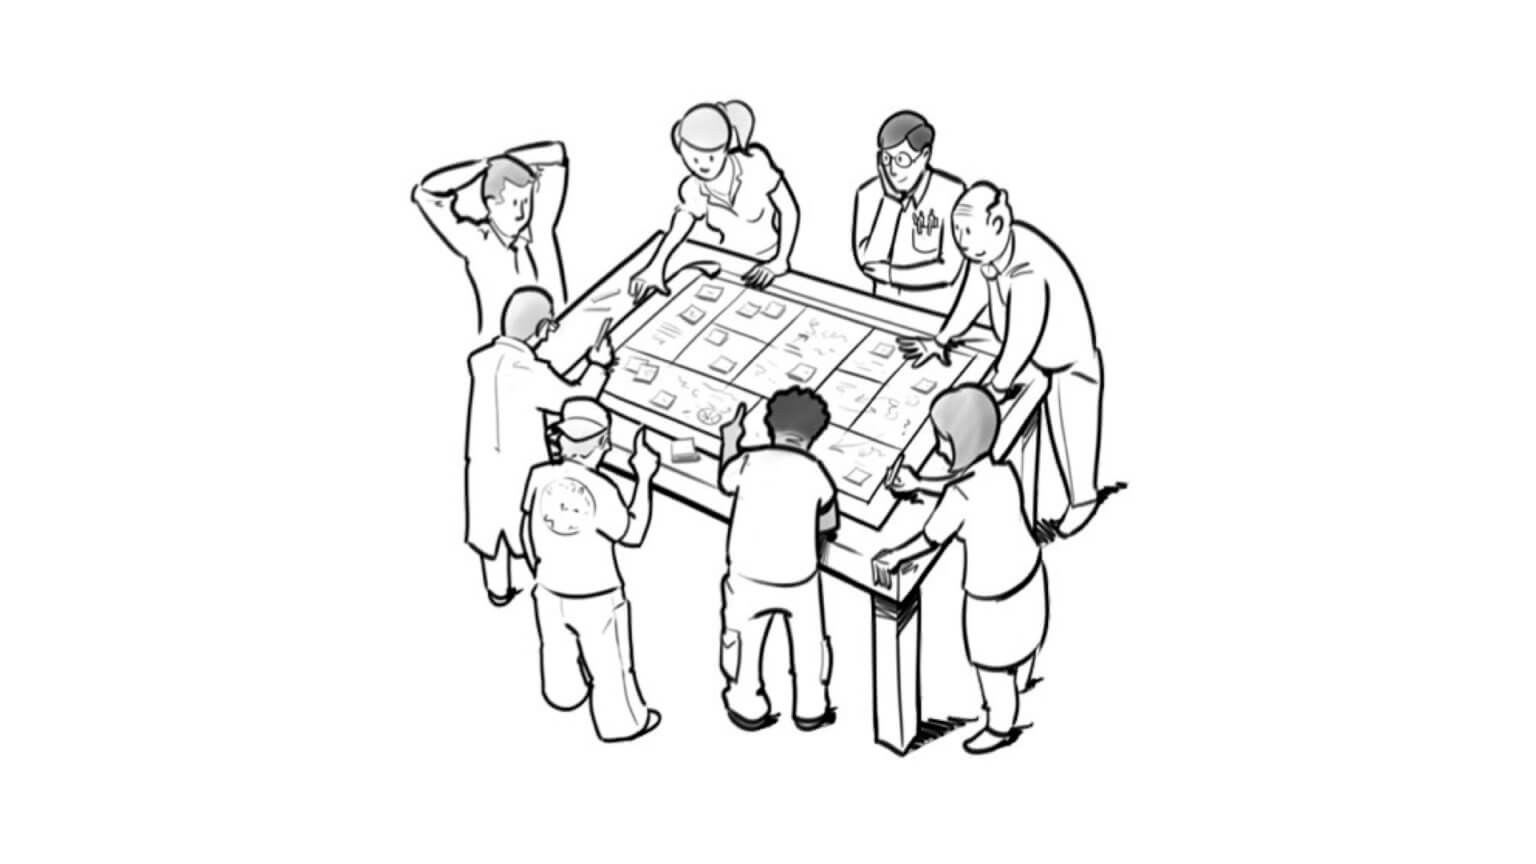
\includegraphics[width=15cm]{images/intro.png}
\end{figure}
\vfill
\pagebreak
% ----------------------- DESENVOLVIMENTO --------------------------
\section{Desenvolvimento}
\subsection{Business Model Canvas - BMC}
\begin{figure}[h]
    \centering
    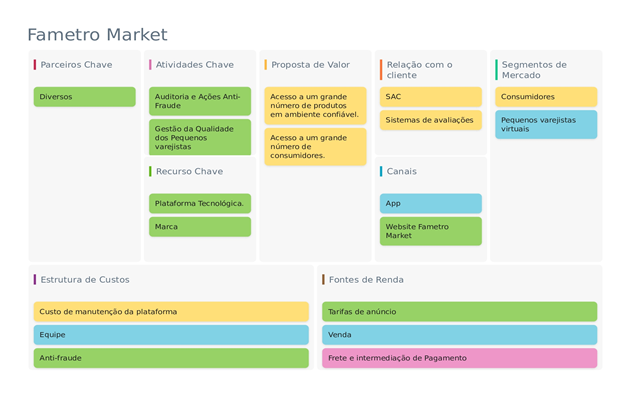
\includegraphics[width=17cm]{images/bmc.png}
    \caption{BMC da empresa ficticia Fametro Marketplace}
\end{figure}
\subsection{Proposta de Valor}
\par Oferecemos um conjunto de soluções e ferramentas para potencializar a capacidade de comprar e vender pela Internet, nosso foco é facilitar e popularizar a compra e venda no Brasil e no mundo, cliente e varejistas podem acessar a plataforma onde poderão gerenciar e compra os produtos disponibilizados no marketplace com isso aumentamos a diversidade de produtos disponibilizados e impulsionar o desenvolvimento de uma comunidade empreendedora. \\

\includegraphics[width=\linewidth/2]{images/proposta-1.png}

\includegraphics[width=\linewidth/2]{images/proposta-2.png}
\subsection{Segmento de Mercado}
\par No mercado de compra e venda online existe dois grandes grupos que se encaixam no modelo de negócio de um marketplace. Depois de analisar minimamente o mercado começamos com o público que quer comprar sem sair de casa e receber as suas encomendas com rapidez e segurança, esses fazem parte do grupo de clientes e para o sucesso do negócio precisamos mapear os seus perfis e traçar a estratégia de marketing mais eficiente e certeira para que possamos oferecer para eles os produto ou serviços que mais se adequam. 
\begin{itemize}
    \item \textbf{{Clientes}}
    \par Analisando o grupo de cliente entendemos que existem pessoas de diferentes gerações e precisamos analisar os principais hábitos de consumo por geração e adequar o modelo de negócio para que as estratégias de marketing tenham sucesso. Atualmente a sociedade conta com quatro gerações de consumidores no mercado. Com essa realidade, é necessário compreender quais são os hábitos de consumo de cada categoria de compradores. Pensando nisso, reunimos alguns detalhes que apontam as principais diferenças comportamentais por geração, conforme seus respectivos anos de nascimento.
    \begin{itemize}
        \item \textbf{Baby Boomers (1945 a 1964)}
        \par Geração que ajudou a impulsionar os modos de consumo de hoje: sem respeito cego às marcas, bem como exigências de diversidade e qualidade. Em geral, só compram aquilo que já viram fisicamente. Ou seja, são aqueles que visitam um estabelecimento para conhecer o produto antes de comprar pela internet.
        \item \textbf{Geração X (1965 a 1984)}
        \par Pessoas conhecidas pelo incentivo à competitividade entre marcas e produtos. Prezam o conforto e a praticidade que as mercadorias e serviços podem oferecer, porém necessitam ser educadas e convencidas antes de comprar.
        \item \textbf{Geração Y ou Millenials (1985 a 1999)}
        \par Indivíduos que vivenciaram a evolução da internet e da tecnologia. Em razão disso, são fáceis de aceitar novidades. Priorizam a instantaneidade, como meios de pagamento digitais e a possibilidade de fazer compras sem sair de casa.
        \item \textbf{Geração Z (2000  a atual)}
        \par São os famosos “nativos digitais”, ou seja, nasceram após o advento da web. Eles compreendem os mecanismos virtuais mais rápido do que as gerações anteriores. Gostam de exclusividade e anseiam que tudo seja resolvido em um único dispositivo.
    \end{itemize}
    \par De posse dos perfis e dados dos clientes podemos traçar uma estratégia de marketing que seja adequada para cada perfil mapeados. Essa segmentação de cliente nos permite sermos mais assertivos e a porcentagem de sucesso aumenta.
    \item \textbf{{Lojistas e Varejistas}}
    \par Agora temos o segundo grupo de segmentação do marketplace que o grupo que irá vender e nesse grupo que precisamos de muita atenção pois eles são um dos parceiros que teremos nessa empreitada por tanto assim como os clientes precisamos oferecer para eles segurança nas suas transações, um gerenciamento do seu negócio detalhado para que ele tenha o controle de estoque, cliente finanças e outro. Mostrar que eles podem vender qualquer produto para qualquer pessoa em qualquer lugar do Brasil e posteriormente no mundo é de extrema importância para o sucesso do nosso marketplace.
\end{itemize}
\subsection{Os Canais}
\par Os canais que usaremos para com nossos clientes são: website do marketplace e pelo app de compra e venda. Temos a responsabilidade de levar a melhor experiência para nossos clientes e parceiros, por isso disponibilizamos canais que eles podem interagir online entre si em tempo real.\\
\begin{center}
    
\includegraphics[width=10cm]{images/canais.png}
\end{center}
\subsection{Relacionamento com os Clientes}
\par Para que nossos cliente e parceiros não se sintam só nessa caminhada disponibilizaremos formas de relacionamento tanto com os clientes como os varejistas que estão em nossa plataforma. Através do \textbf{SAC (Serviço de atendimento ao consumidor)} nossos parceiros poderão entrar em contato conosco para tirar suas dúvidas e também estaremos atento as suas reclamações através de nossos sistemas de atendimento personalizados, para que a plataforma esteja em constante melhoria, atualização e evolução. Também disponibilizaremos \textbf{sistema de avaliação}, no qual, os clientes e lojistas poderão avaliar a plataforma de forma clara e rápida. Essa forma de relacionamento com nossos parceiros é de extrema importância para nós, pois é através desse sistema que saberemos se estamos atingindo nosso objetivo para com clientes.\\

\includegraphics[width=\linewidth/2]{images/rel-cliente-1.png}

\includegraphics[width=\linewidth/2]{images/rel-cliente-2.png}
\subsection{Atividade-Chave}
\par Neste ponto mostraremos as atividades que darão suporte a nossa \textbf{proposta de valor} e para o sucesso do nosso modelo de negócio implantaremos meios para a segurança de transações e processos que jugamos importante para que o nosso desafio de entregar uma plataforma segura, antifraude e de qualidade para nossos clientes seja concluída.
\par Primeiramente implantaremos métodos que evitem fraudes em nossos sistemas por meio de sistemas antifraude que podem ser desenvolvidos por empresas terceirizadas. Em seguida implantaremos processos de auditoria interna para garantir que nossos processos estejam de acordo com normas e procedimentos de segurança estabelecidos pela ISO 27001 que é a norma de segurança de informação, garantindo assim que nosso sistema de gestão de dados e atendimento, transações, compra e venda estejam todos validade e homologado perante as ISOS que nos permite atuar em nosso segmento de atuação. Logo abaixo falaremos um pouco sobre o que a fraude e auditoria interna para que fique claro o desafio que temos pela frente.
\begin{itemize}
    \item \textbf{{Fraude}}
    \par A fraude pode ser definida como qualquer ato ilegal caracterizado por engano, ocultação ou violação de confiança. Tais atos não dependem da ameaça de violência ou força física. Fraudes são executadas por partes e organizações para obter dinheiro, propriedades ou serviços; para evitar pagamento ou perda de serviços; ou para garantir vantagem pessoal ou comercial. A fraude não é exclusividade de qualquer tipo de organização. Ocorre em empresas públicas e privadas, sem fins lucrativos, em organizações que buscam contribuir para o bem-estar econômico e social, como departamentos governamentais, instituições financeiras, e serviços públicos e privados (água, eletricidade, educação, saúde, etc.). Em suma, a oportunidade de cometer fraude existe em todos os setores. A forma como as organizações lidam com o risco de fraude pode ser influenciada pela jurisdição legal e pela avaliação de riscos e apetite a risco da própria organização. A fraude pode, frequentemente, levar a litígio, demissões e recuperação de ativos. É essencial, portanto, que qualquer investigação seja realizada por indivíduos devidamente qualificados, para reduzir o risco de comprometer as evidências, fazer acusações indevidas ou prejudicar possíveis ações legais. Em conformidade com as Normas Internacionais para a Prática Profissional de Auditoria Interna do The IIA sobre proficiência (1210.A2), os auditores internos devem ter conhecimento suficiente para avaliar o risco de fraude e a maneira pela qual ele é gerenciado pela organização.
    \item \textbf{{Auditoria interna}}
    \par A auditoria interna é uma atividade independente e objetiva de avaliação e consultoria, criada para agregar valor e melhorar as operações da organização. Seu papel inclui detectar, prevenir e monitorar os riscos de fraude e abordar esses riscos em auditorias e investigações. Deve-se considerar onde o risco de fraude está presente no negócio e responder apropriadamente, auditando os controles dessa área, avaliando o potencial de ocorrência de fraude e como a organização gerencia o risco de fraude (Norma 2120.A2) por meio da avaliação de riscos e do planejamento de auditoria. Não é responsabilidade direta da auditoria interna impedir que fraudes ocorram na empresa. Essa é uma responsabilidade da administração como primeira linha de defesa. Não se deve esperar que o auditor interno tenha a experiência de uma pessoa cuja responsabilidade primária seja investigar fraudes. Tais investigações são realizadas com melhor qualidade por aqueles experientes para executar tais tarefas. A auditoria interna deve usar sua expertise para analisar conjuntos de dados para identificar tendências e padrões que possam sugerir fraudes e abusos de financiamento. Quando não houver experiência disponível na equipe de auditoria interna, a organização deve considerar recrutar ou alocar recursos com conhecimento ou experiência suficiente. A organização deve ter um plano de resposta antifraude adequado, que delineie as principais políticas e metodologias de investigação. O plano deve deixar claro o papel da auditoria interna em casos de suspeita de fraude e falhas associadas de controle.
\end{itemize}
\par Dados os conceitos acima sobre fraude e auditoria, por fim abordaremos agora o último ponto que precisamos implantar para o sucesso do modelo que é a  \textbf{gestão da qualidade dos pequenos varejistas.} Que nos permitirá gerenciar todos os nossos parceiros lojistas para que tenhamos uma clara visão sobre o negócio de cada um deles e assim poder atendê-los da melhor maneira com as melhores serviços e ferramentas. 
\subsection{Recursos Principais}
\par Nesta parte do modelo de negócio temos o desafio de mostrar os recursos principais para que consigamos de fato lança a plataforma. Abaixo mostraremos quais são:
\begin{itemize}
    \item \textbf{Plataforma tecnológica}
    \par A nossa plataforma terá que se manter atualizadas com as tecnologias mais atuais mercado para que sejamos líder no em nosso seguimento implementaremos recursos e tecnologias que nos ajudaram a nos manter na frente, estudos e pesquisa estão sendo feitas para identificarmos tais ferramentas, após termos conhecimentos sobre elas implementaremos e integraremos com nosso ambiente de soluções para que possamos estar interconectados.
    \item \textbf{Marca}
    \par A marca é um ponto muito importante, pois será ela que chegar até nossos clientes (compradores e lojistas parceiros). A presença da nossa marca carregará todos os nossos princípios e valores bem como nossa missão e objetivo. Para que nossa marca seja conhecida de forma positiva participaremos de workshops, palestras e mentorias para que possamos obter todo o \textbf{know-how} que necessitamos para criar uma marca forte e que passe segurança e confiança para todos. O conhecimento e sobre o negócio de marketplace é importante para nosso avanço bem como contratar pessoas que possuem tais conhecimentos e experiências nos ajudará a chegar mais rápido em nossas metas.
\end{itemize}
\subsection{Parcerias Principais}
\par Como nosso negócio de atuação é bem amplo devemos nos atentar para formamos parcerias que nos tragam rapidez e segurança nos nossos trabalhos do dia-dia. Em nosso Canvas adicionamos o post it de diversos mostrando assim que a estamos abertos a várias parcerias que nos levaram a um outro nível. Tais parceiros serão analisados e os que estiverem de acordo com os objetivos e valores serão integrados em nosso ecossistema empresarial. 
Provavelmente teremos parceiros na parte de infraestrutura e toda parte de servidores de Cloud Computer, nossas redes, citando alguns como Microsoft Azure, Amazon AWS entre outros.\\[1cm]

\includegraphics[width=\linewidth/2]{images/parceria-1.png}

\includegraphics[width=\linewidth/2]{images/parceria-2.png}
\subsection{Fontes de Receita}
\par Para que toda nossa estrutura se mantenha precisamos de fontes de renda e monetizar o nosso modelo para que possa nossas operações permaneçam ativas. Para isso temo 3 pontos no qual estruturamos para nos atender financeiramente. São elas: 
\begin{itemize}
    \item \textbf{Tarifas de anúncio}
    \par Teremos nossas taxas aplicadas aos anúncios realizados pelos nossos parceiros varejistas. Tarifas essas que serão praticadas dependendo do tipo de anúncio que o lojista queira veicular através de nossa plataforma.
    \item \textbf{Venda}
    \par Através das vendas realizadas em nossas plataformas obteremos um valor que será direcionado para pagar os custos e mantermos nossos administrativo funcionando perfeitamente.
    \item \textbf{Frete e intermediação de pagamento}
    \par Fretes e pagamentos também serão taxados com um percentual equivalente e justo para que as duas partes lucrem e dessa forma manter a parceira por mais tempo e assim mantendo a plataforma ativa para todos que desejarem negociar através dela.
\end{itemize}
\par Por fim deixamos claro que as taxas praticadas por nós terão que ser feitas mediantes cláusulas de contrato para assegurar que as duas partes estejam cientes do que foi acordado. Lembrando que não cobraremos de nossos clientes (lojistas e varejista) taxas para que criem suas lojas e utilizem a nossa plataforma, por isso a importância de termos uma estrutura de fontes e receitas para que mantenhamos nossas operações e garantindo o lucro de nossos investidores.
\subsection{Estrutura de Custos}
\par Teremos custos pontuais como:
\begin{itemize}
    \item \textbf{Custo de manutenção da plataforma}
    \par Desenvolvimento de ferramentas, manutenção de maquinas e outras.
    \item \textbf{Equipe} 
    \par Custo de pessoal, custos com material entre outros
    \item \textbf{Sistemas antifraude}
    \par Sistemas que são de fundamental importância para o funcionamento correto de nossa plataforma. Podem ser desenvolvida internamento por uma equipe de tecnologia ou poderá ser adquirida de empresas terceirizadas.
\end{itemize}
\par Para que nos mantenhamos ativos no mercado tais custos terão que ser abatido com as receitas que estruturamos no tópico anterior.
\vfill
\pagebreak
% ----------------------- CONCLUSÃO --------------------------
\section{Conclusão}
\par Portanto concluo assim nosso modelo de negócio que será de marketplace, através dos tópicos acima mostramos como será nossa atuação no mercado e de que modo faremos. Tais métodos, processos e ferramentas nos ajudaram a nos aproximar de nosso objeto que é o de ter um modelo validado e aplicado junto a nossos clientes e podermos ter sucesso e o lucro esperado.

\vfill
\pagebreak
% ----------------------- BIBLIOGRAFIA --------------------------
\section{Bibliografia}
\begin{itemize}
    \item The Institute of Internal Auditors - \textbf{DECLARAÇÃO DE POSICIONAMENTO DO IIA - FRAUDE E A AUDITORIA INTERNA}. Ed. única. Lake Mary, EUA.

    \item Segmentação de Público: Você está vendendo para as pessoas certas, TrayCorp, 2019. Disponível em: \textbf{\\https://www.traycorp.com.br/segmentacao-publico-ecommerce/}. 
    \\Acesso em 30 de outubro de 2021.
    
    \item Quer Aplicar O Business Model Canvas? Veja Alguns Exemplos, ABStartUps, 2019. Disponível em: \textbf{\\abstartups.com.br/quer-aplicar-o-business-model-canvas-veja-alguns-exemplos}. 
    \\Acesso em 30 de outubro de 2021.
    
    \item O que é o Business Model Canvas, Analista de Modelos de Negócio, 2018. Disponível em: \textbf{\\ https://analistamodelosdenegocios.com.br/o-que-e-o-business-model-canvas/}.
    \\Acesso em 25 de outubro de 2021.
\end{itemize}
\end{document}
